\documentclass[a4paper,12pt]{article}
\usepackage[utf8]{inputenc}
\usepackage{graphicx}
\usepackage[hidelinks]{hyperref}
\usepackage{amsmath}
\usepackage[a4paper, left=2cm, right=2cm, top=3cm, bottom=3cm]{geometry}
\usepackage{titlesec}
\usepackage{listings}
\usepackage{color}
\usepackage{courier} 

\title{Informe de Auditoría del Sistema Web}
\date{}  % Se deja vacío para no mostrar la fecha en la portada

% Cambiar los títulos de los índices
\renewcommand{\contentsname}{Índice de Contenidos}
\renewcommand{\listfigurename}{Índice de Figuras}
\renewcommand{\listtablename}{Índice de Tablas}

\renewcommand{\figurename}{Figura}

\newcommand{\cita}[1]{\textit{``#1''}}

\newcommand{\code}[1]{\texttt{#1}}  % Comando para uso en línea (sin formato de bloque)

% Configuración para bloques de código
\lstset{
	basicstyle=\ttfamily\small\color{black}, % Fuente monoespaciada y color negro
	keywordstyle=\color{blue}\bfseries,      % Color para palabras clave
	commentstyle=\color{gray},               % Color para comentarios
	stringstyle=\color{purple},              % Color para cadenas de texto
	showstringspaces=false,                  % Oculta los espacios en las cadenas
	frame=single,                            % Marco alrededor del código
	breaklines=true,                         % Línea nueva para evitar desbordamiento
	captionpos=b,                            % Posición de la leyenda (abajo)
}

% Comando para insertar bloques de código con estilo personalizado
\newcommand{\codeblock}[1]{\begin{lstlisting}#1\end{lstlisting}}




\begin{document}
	\maketitle
	\vfill  % Esto empuja el contenido hacia el final de la página.
	\begin{flushright}  % Alinea el texto a la derecha
		\textbf{Integrantes del grupo:} \\[0.5em]
		Jorge Illera Rivera \\[0.5em]
		Iker Argulo Galán \\[0.5em]
		Oscar Lijerón Pérez \\[0.5em]
		Bruno Izaguirre Martínez de Marañón \\[0.5em]
		María Bogajo \\[0.5em]
		Ander Javier Corral \\[0.5em]
		\textbf{Fecha:} \\[0.5em]
		09/11/2024
	\end{flushright}
	\newpage
	

\tableofcontents
\listoffigures
\listoftables
\newpage

\section{Introducción}
Este informe detalla la auditoría de seguridad del sistema web utilizando OWASP ZAP, con el objetivo de identificar y mitigar vulnerabilidades.

\section{Metodología}
La auditoría se realizó mediante un análisis de ZAP, ejecutando... 

\section{Vulnerabilidades}


\subsection{Rotura de control de acceso}
\subsubsection{Soluciones implementadas}



\subsection{Fallos criptográficos}
\subsubsection{Soluciones implementadas}



\subsection{Inyección}
En la sección de inyección se ha identificado una amenaza de alto riesgo. La vulnerabilidad detectada corresponde a un ataque de Cross-Site Scripting (XSS), como se puede observar en la Figura \ref{fig:xss_error}.
\begin{figure}[h]
	\centering
	\fbox{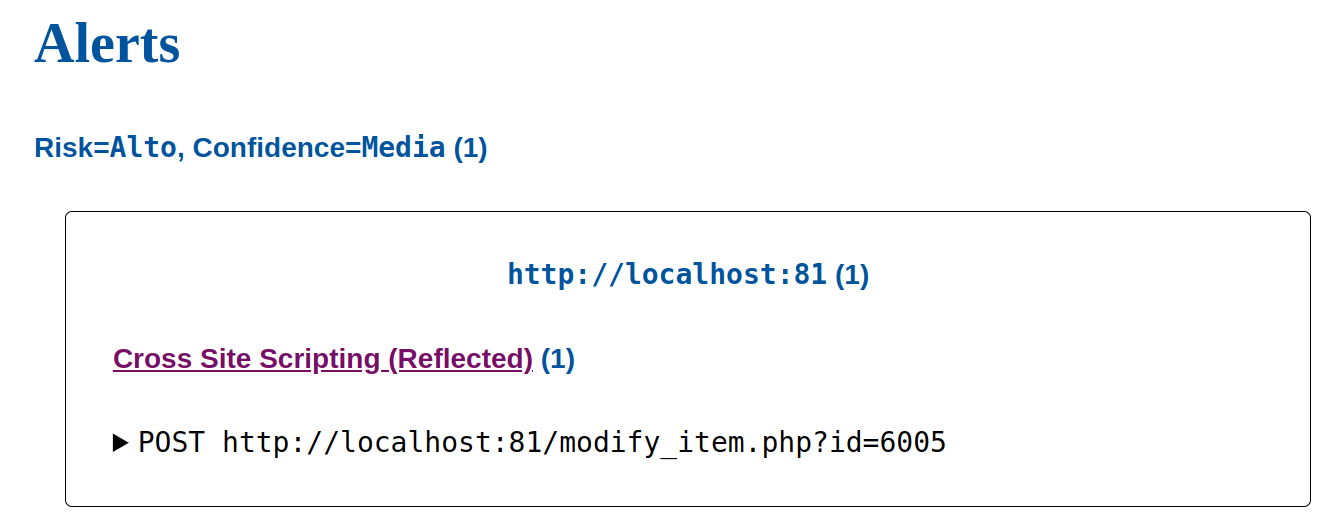
\includegraphics[width=0.7\textwidth]{figures/injection-error.png}} % Imagen con borde negro
	\caption{Errores de inyección detectados por ZAP.}
	\label{fig:xss_error}
\end{figure}

\subsubsection{Cross-Site Scripting (XSS)}
La vulnerabilidad CWE-79 corresponde a Cross-Site Scripting (XSS) Reflejado, que permite a un atacante inyectar código malicioso en los parámetros de entrada del sistema, como los campos de formularios o las URL. Cuando un usuario accede a una URL o un formulario que contiene este código inyectado, el navegador del usuario ejecuta dicho código, lo que puede llevar a la manipulación de datos, el robo de cookies, la ejecución de scripts no autorizados, y otros ataques de seguridad.

\textbf{Causa de la vulnerabilidad}

La vulnerabilidad XSS detectada se originaba en el archivo \code{modify\_item.php}, más concretamente en el campo de la fecha de lanzamiento y en otros campos de entrada en el formulario de modificación de un juego. Esto se debía a que los valores de entrada eran reflejados en la respuesta sin la sanitización o validación adecuada, permitiendo a los atacantes inyectar y ejecutar código JavaScript en el navegador del usuario.

\textbf{Pruebas y comportamiento observado}

Sin la sanitización de entrada: OWASP ZAP detectó que ciertos campos permitían la inyección de código JavaScript en los valores de los formularios.\\ Por ejemplo, en el campo de la fecha, se podía ingresar un valor como \\\code{<script>alert(1);</script>}, lo cual provocaba la ejecución de un alert en el navegador.


\textbf{Conclusiones}

La vulnerabilidad de XSS reflejada fue una amenaza crítica para la aplicación, ya que podía permitir a los atacantes ejecutar código malicioso en el navegador de los usuarios. Gracias a la implementación de sanitización y validación estrictas en los campos de entrada y salida, esta vulnerabilidad se ha mitigado de manera efectiva. La aplicación ahora cumple con un estándar de seguridad más alto, protegiendo los datos y la experiencia de los usuarios frente a posibles ataques de inyección de código.

\subsubsection{Soluciones implementadas}
Para mitigar la vulnerabilidad de XSS y otros posibles ataques de inyección, se implementaron las siguientes soluciones:

\begin{itemize}
	\item \textbf{Sanitización de entrada y escapado de salida:\\}
	Se utilizó la función \code{htmlspecialchars()} en PHP para escapar caracteres especiales (como <, >, \&, ", ') en todas las salidas. Esto asegura que el contenido reflejado en el navegador sea tratado como texto y no como código ejecutable.
	
	\item \textbf{Validación y sanitización de fecha de lanzamiento:\\} Se implementó una expresión regular (\code{preg\_match}) para asegurarse de que las fechas ingresadas cumplan con el formato \code{YYYY-MM-DD}.
	
	\item \textbf{Sanitización de datos entrantes:\\} Para cada valor de entrada recibido a través del formulario, se aplicó \\ \code{mysqli\_real\_escape\_string()} para evitar que cualquier código especial o malicioso llegue a la base de datos.
	
	\item \textbf{Validación de Campos Numéricos (rating y price):\\} Los valores de rating y price se convirtieron a tipo float usando \code{floatval()} para asegurarse de que se almacenan y procesan correctamente como valores numéricos.
\end{itemize}

\textbf{Resultados de la Segunda Auditoría}

Después de implementar las soluciones descritas, se realizó un segundo análisis con OWASP ZAP. Los resultados fueron positivos: no se detectaron vulnerabilidades de XSS ni otros problemas de inyección.


\subsection{Diseño inseguro}
\subsubsection{Soluciones implementadas}



\subsection{Configuración de seguridad insuficiente}
\subsubsection{Soluciones implementadas}



\subsection{Componentes vulnerables y obsoletos}
\subsubsection{Soluciones implementadas}



\subsection{Fallos de identificación y autenticación}
\subsubsection{Soluciones implementadas}



\subsection{Fallos en la integridad de datos y software}
\subsubsection{Soluciones implementadas}



\subsection{Fallos en la monitorización de la seguridad}
\subsubsection{Soluciones implementadas}



\section{Conclusiones}




\section{Bibliografía}
\begin{thebibliography}{9}
	\bibitem{owasp-xss} OWASP, "Cross-Site Scripting (XSS)", https://owasp.org/www-community/attacks/xss/, accedido el 3 de noviembre de 2024.
\end{thebibliography}




\section{Apéndices}


\end{document}

